% !TEX encoding = UTF-8 Unicode
\documentclass[a4paper]{article}

\usepackage{color}
\usepackage{url}
\usepackage[T2A]{fontenc} % enable Cyrillic fonts
\usepackage[utf8]{inputenc} % make weird characters work
\usepackage{graphicx}
\usepackage[english,serbian]{babel}
%\usepackage[english,serbianc]{babel} %ukljuciti babel sa ovim opcijama, umesto gornjim, ukoliko se koristi cirilica

\usepackage[unicode]{hyperref}
\hypersetup{colorlinks,citecolor=green,filecolor=green,linkcolor=blue,urlcolor=blue}

\usepackage{listings}

%\newtheorem{primer}{Пример}[section] %ćirilični primer
\newtheorem{primer}{Primer}[section]

\definecolor{mygreen}{rgb}{0,0.6,0}
\definecolor{mygray}{rgb}{0.5,0.5,0.5}
\definecolor{mymauve}{rgb}{0.58,0,0.82}

\lstset{ 
  backgroundcolor=\color{white},   % choose the background color; you must add \usepackage{color} or \usepackage{xcolor}; should come as last argument
  basicstyle=\scriptsize\ttfamily,        % the size of the fonts that are used for the code
  breakatwhitespace=false,         % sets if automatic breaks should only happen at whitespace
  breaklines=true,                 % sets automatic line breaking
  captionpos=b,                    % sets the caption-position to bottom
  commentstyle=\color{mygreen},    % comment style
  deletekeywords={...},            % if you want to delete keywords from the given language
  escapeinside={\%*}{*)},          % if you want to add LaTeX within your code
  extendedchars=true,              % lets you use non-ASCII characters; for 8-bits encodings only, does not work with UTF-8
  firstnumber=1000,                % start line enumeration with line 1000
  frame=single,	                   % adds a frame around the code
  keepspaces=true,                 % keeps spaces in text, useful for keeping indentation of code (possibly needs columns=flexible)
  keywordstyle=\color{blue},       % keyword style
  language=Python,                 % the language of the code
  morekeywords={*,...},            % if you want to add more keywords to the set
  numbers=left,                    % where to put the line-numbers; possible values are (none, left, right)
  numbersep=5pt,                   % how far the line-numbers are from the code
  numberstyle=\tiny\color{mygray}, % the style that is used for the line-numbers
  rulecolor=\color{black},         % if not set, the frame-color may be changed on line-breaks within not-black text (e.g. comments (green here))
  showspaces=false,                % show spaces everywhere adding particular underscores; it overrides 'showstringspaces'
  showstringspaces=false,          % underline spaces within strings only
  showtabs=false,                  % show tabs within strings adding particular underscores
  stepnumber=2,                    % the step between two line-numbers. If it's 1, each line will be numbered
  stringstyle=\color{mymauve},     % string literal style
  tabsize=2,	                   % sets default tabsize to 2 spaces
  title=\lstname                   % show the filename of files included with \lstinputlisting; also try caption instead of title
}

\begin{document}

\title{Haskell: Debagovati ili nedebagovati?\\ \small{Seminarski rad u okviru kursa\\Metodologija stručnog i naučnog rada\\ Matematički fakultet}}

\author{Vladimir Batoćanin, Stefan Stefanović, Jovan Lezaja, Đorđe Jovanović}

%\date{9.~april 2015.}

\maketitle

\abstract{
U ovom tekstu je ukratko prikazana osnovna forma seminarskog rada. Obratite pažnju da je pored ove .pdf datoteke, u prilogu i odgovarajuća .tex datoteka, kao i .bib datoteka korišćena za generisanje literature. Na prvoj strani seminarskog rada su naslov, apstrakt i sadržaj, i to sve mora da stane na prvu stranu! Kako bi Vaš seminarski zadovoljio standarde i očekivanja, koristite uputstva i materijale sa predavanja na temu pisanja seminarskih radova. Ovo je samo šablon koji se odnosi na fizički izgled seminarskog rada (šablon koji \emph{morate} da koristite!) kao i par tehničkih pomoćnih uputstava. Pročitajte tekst pažljivo jer on sadrži i važne informacije vezane za zahteve obima i karakteristika seminarskog rada.}

\setcounter{tocdepth}{1} % show only sections in table of contents
\tableofcontents

\newpage

\section{Uvod}
\label{sec:uvod}

{Dizajn programskog jezika Haskell je takav da programerovo vreme provedeno za kodom je manje debagujući, a više trudeći se da inicijalno napiše ispravan i robustan kod. Ovo stanovište se može braniti činjenicom da je Haskell čist funkcionalni jezik, što znači da je dosta pouzdana praksa izolovano testiranje svake funkcije, kao i stroga tipiziranost, koja drastično smanjuje šansu da se programer vrati na prethodno napisani deo koda. 
\\ \\
Ovo u idealnim slučajevima važi, s tim što ovo ne uključuje slučaj gde programer napravi semantičku grešku koja prolazi fazu prevodjenja, kao i slučajeve gde potpisi funkcija nisu ispravni, nisu potpuni ili su prosto nepostojeći. Ovo sve dovodi do odloženih rafalnih grešaka ili do pojave teško uočljivih bagova. Tada nam je potreban neki metod da i otkrijemo uzrok te greške da bismo je i otklonili.}

\section{Matematičko dokazivanje}

Za funkcionalnu paradigmu se veoma lako nalazi analogon na formalno matematičkom jeziku, što nam dozvoljava da već u fazi inicijalnog pisanja koda dokažemo da je naš program matematički korektan. U ovom kontekstu se najčešće koristi metod {\em struktruralne indukcije}  (eng.~{\em structural induction}). Ovo je moguće isključivio zbog rekurzivno definisanih struktura podataka u Haskell-u, pri čemu se koristi operator | (ili) koji označava matematičku uniju.
\begin{lstlisting}[caption={Rekurzivno definisanje liste u Haskellu},frame=single, label=simple]
data Lista x = PraznaLista | Cons a (Lista x)
\end{lstlisting}
Znajući ovo, vrlo lako možemo dokazati korektnost programa koji koriste liste uz pomoć matematičke indukcije, gde bi nam baza indukcije bio slučaj prazne liste, a induktivni korak rekurzivni poziv liste koju dobijamo dodajuci neki broj elemenata na listu za koju pretpostavimo da važi funkcija na osnovu induktivne hipoteze, kao na primer:
\begin{lstlisting}[caption={Primer rekurzivno definisane funkcije},frame=single, label=simple]
sum :: [Int] -> Int
-- baza indukcije
sum [] = 0
-- induktivna hipoteza koja vazi za xs
-- induktivni korak dodavanja jednog elementa x na xs
sum (x:xs) = x + sum xs 
\end{lstlisting}


\section{GHCi Debager}
GHCi debager nam omogućava da u željenim momentima zaustavimo program i proverimo vrednosti pojedinačnih promenljivih preko {\em tačaka zaustavljanja} (eng.~{\em breakpoints}). Takodje vrlo bitna funkcionalnost je korak-po-korak izvršavanje programa sa zaustavljanjem. Izuzetak od ove funkcionalnosti su vec prekompilirane importovane biblioteke u koje nije moguće ući u okviru međukoraka.


\subsection{Tačke zaustavljanja i inspekcija varijabli}
Iako je moguće zaustaviti program na bilo kom izrazu odnosno liniji radi inspekcije varijabli, nije moguće proveriti tip i vrednost varijabli koje već nisu izračunate. Ovo je posledica činjenice da se u Haskellu ne vrši zaključivanje tipova tokom izvršavanja programa. Naravno, uvek je moguće forsirati dedukcije tipa, odnosno naterati program da nastavi izvršavanje taman toliko da usko odredi sa kojim tipom podataka se radi. Problem kod ovog pristupa se javlja u slučajevima kada bismo u bloku koda koji treba da se izvrši da bismo dobili definitni tip željene promenljive postoji ugnježdena tačka zaustavljanja, što uništava linearnost inspekcije i debagovanja koda. 

Posledice ovog problema se mogu amortizovati uvođenjem parcijalnog izračuvanja tipa izraza, umesto izračunavanja vrednosti celog izraza. Kao i uvodjenje posebne komande za ispisivanje jos neevaluiranih vrednosti, ovo je vrlo korisno s obzirom da svaki tip pre nego što može konvencionalno da se ispisuje mora da ima implementiranu funckiju za prikazivanje (eng. {\em show}). Neevaluirane vrednosti Haskell rešava uvođenjem {\em obećanja} (eng. {\em thunk},Learn You a Haskell for Great Good), koje se uvek koriste pri lenjom izračunavanju. Nedostatak ove implementacije je to što bilo koji izraz koji se lenjo odseče i ne izračuna se do kraja (na primer desna strana izraza konjukcije gde je prvi argument{\em False}), što znači da ni obećanje koje se nalazilo u odsečenom delu izraza nikada neće biti evaluirano. 


\subsection{Trace}

U tradicionalnim nefunckionalnim jezicima se podrazumeva postojanje debagera, koji prati tačnu sekvencu poziva koji su se izvršavali od pokretanja programa. Ovo je izutetno teško implementirati u programskim jezicima kao što je Haskell zbog toga što se izrazi i funkcije ne izračunavaju tačnim redosledom kojim su pozvani već se izračunavaju tek kada su potrebni za neko drugo izračunavanje (eng. {\em demand-driven execution}). Idealno rešenje bi bilo da se programera apstrahuje evaluacija koja bi izgledala što više kao ona u imperativnom jeziku, dok bi interno bio čuvan pravi redosled poziva i evaluacija, ovo rade neki Haskell debageri, ali GHCi nema tu funkcionalnost, odnosno ne pravi leksicki stek poziva (eng. {\em lexical call stack}) , on nam isključivo daje da na tackama zaustavljanja imamo pregled prethodnih koraka evaluiranja.
%TODO: dodati sajt u source za demand-driven execution: https://downloads.haskell.org/~ghc/7.6.3/docs/html/users_guide/ghci-debugger.html


\section{Debagovanje korišćenjem Heta}
Het (eng. {\em Hat -- {\bf \em Ha}skell {\bf \em t}racer}) je alat koji se koristi za generisanje {\em traga} (eng. {\em trace}) prilikom izvršavanja Haskel programa
i nadziranje tako generisanog {\em traga} \cite{chitil2002transforming}. Smatra se jednim od najnaprednijih alata za debagovanje u Haskelu. Prednost alata Het u odnosu na ostale alate za debagovanje 
se ogleda upravo u upotrebi {\em traga}, jer se programeru pruža pogled unutar ``crne kutije'', tj. sva izračunavanja u našem Haskel programu bivaju razmotana u niz redukcija koja programer može da analizira korišćenjem različitih interaktivnih alata, pri čemu svaki od njih na različite načine interpretira generisane tragove i omogućava široki spektar analiza izračunavanja Haskel programa.
Ovaj alat nije deo nekog prevodioca ili interpretatora za programski jezik Haskel,
što se moglo smatrati prednošću u vremenu kada se su se koristili različiti prevodioci za Haskel programski jezik, pa samo njegovo postojanje i održavanje nije bilo tesno vezano za postojanje i održavanje nekog specifičnog prevodioca, odnosno interpretatora \cite{chitil2002transforming}. Međutim danas, u vremenu kada je {\em GHC} ({\em GHC -- Glasgow Haskell Compiler}) najpristupačniji Haskell prevodilac, ta osobina Heta ne mora da se nužno smatra prednošću, uzimajući u obzir da se sa konstantnim izlaskom novih verzija {\em GHC}-a javlja potreba za konstantnim održavanjem.
U ovom radu naglasak će biti na korišćenju alata Het kao debagera, no on može da se koristi i u svrhe posmatranja kako funkcioniše korektno napisan Haskel program \cite{wallace2001multiple}.
Nažalost, usled zastarelosti biblioteka koje koristi alat Het, autori rada nisu uspeli da osposobe alat na svojim mašinama nakon više pokušaja. 
%TODO: ovde bi trebalo dodati rečenicu koja naglašava da debagovanje u Haskelu samim tim nije bas ``najudobnije'', makar sto se tice Heta 
%TODO: najveća mana Heta to što nije podržan u novijim verzijama. manjak dokumentacije ga čini nepristupačnim itd.

Alat Het pruža programeru uvid u detalje izračunavanja pri izvršavanju Haskel programa korišćenjem {\em tragača} (eng. {\em tracer}). 
Korišćenjem informacija koje generiše {\em tragač} je moguće locirati greške u našem kodu (ukoliko takvih ima).
Sleđenje {\em tragova} izračunavanja u Hetu se sastoji iz dve faze: prva je {\em ostavljanje traga} (eng. {\em trace generation}), a druga je {\em pregledanje traga} (eng. {\em trace viewing}) \cite{chitil2002transforming}.

\subsection{Ostavljanje traga}
U fazi {\em ostavljanja traga} se pokreće program koji treba da se debaguje tako da ispisuje {\em trag} u određenu datoteku. Da bi program ispisivao {\em trag} u datoteku,
potrebno ga je prvo transformisati korišćenjem alata koji se sadrži u Hetu pod nazivom {\em hat-trans}. U tom procesu se naš Haskel program transformiše u
Haskel program koji se prevodi i linkuje sa odgovarajućim bibliotekama koje pruža Het \cite{chitil2002transforming}. Tako transformisan program se prevodi i pokreće,
pri čemu transformisan program radi isto što i originalni program, uz dodatak da ispisuje {\em trag} u određenu datoteku. % Primećujemo nekoliko razlika u odnosu na ostale debagere.
Jedna od razlika koja se javlja kod Heta u odnosu na neke druge debagere je ta da je uloga transformisanja izvornog koda prepuštena računaru, tj. da je programer oslobođen od dodavanja novog koda u cilju debagovanja, kao što to imamo kod Hud (eng. {\em Hood}) debagera ubacivanjem {\em observe} ključne reči.
Ta osobina alata Het se može smatrati vrlinom, uzimajući u obzir da je cilj debagovanja da bude što ``bezbolniji'' po originalni izvorni kod, kao i po programera, jer menjanje koda ručno donosi još jedan mogući faktor greške. 
Takođe, prilikom pokretanja tako transformisanog programa, datoteku sa tragom je moguće koristiti neograničen broj puta, s obzirom da je ta datoteka sačuvana u sekundarnoj memoriji ne bi li moglo da se koristi više alata iz Heta u jednom pokretanju programa.
Po pitanju zauzetosti memorije ova osobina nije baš poželjna jer, u slučaju debagovanja kompleksnijih programa, datoteka koja sadrži trag izvršavanja programa može da bude velika u smislu memorije.
Nakon ove faze se prelazi u fazu {\em pregledanja traga}.

\subsection{Pregledanje traga}
Kada je naš program završio, moguće je pregledati {\em trag} korišćenjem alata koje nudi Het. Važno je napomenuti da se pod ``završavanje programa'' ne smatra 
da je program isključivo završio {\em ispravno}, već da je program eventualno završio sa nekom porukom o grešci ili pak da je prekinut od strane programera \cite{hat_haskell_org}.
Za analizu {\em traga} Het nudi nekolicinu interaktivnih alata koji pregledaju ponašanje programa, 
između ostalog su to: {\em hat-observe}, {\em hat-trail}, {\em hat-detect}, {\em hat-explore} i {\em hat-stack}. Opis navedenih alata se nalazi u tabeli \ref{tab:tabela_hat}.
Veliki broj alata koji nude različite poglede na program koji se debaguje je jedna od glavnih osobina alata Het, a uzimajući u obzir da su određeni alati inspirisani nekim već postojećim debagerima (Freja (eng. {\em Freja}) kao inspiracija za {\em hat-detect} i Hud (eng. {\em HOOD}) kao inspricija za {\em hat-observe} \cite{hat_haskell_org}), potreba za drugim alatima pri debagovanju je smanjena.

Nažalost, nekompatibilnost alata Het sa novijim verzijama Haskel biblioteka i {\em GHC}-om ({\em GHC} - {\em Glasgow Haskell Compiler}) ga čini nepristupačnim programerima 
koji žele da posvete što manje vremena na iscrpna podešavanja verzija raznoraznih biblioteka, a što više na debagovanje.

\begin{table}[h!]
\begin{center}
\caption{Opis nekih od alata koje nudi Het}
\begin{tabular}{|c|c|} \hline
Naziv alata & Opis\\ \hline
{\em hat-observe} & { Prikazuje kako se koriste funkcije najvišeg nivoa, } \\ & 
		    { tj. za svako ime funkcije prikazuje sve argumente } \\ & 
		    { sa kojima je data funkcija pozivana u toku izračunavanja }\\ & 
		    { programa, kao i rezultate tih poziva \cite{hat_haskell_org}.}\\ \hline
{\em hat-trail} & { Omogućava praćenje izračunavanja {\em unatraške}, } \\ & 
		  { počevši od poruke o grešci ili od izlaza programa \cite{hat_haskell_org}.}\\ \hline
{\em hat-detect} & { Postavljanjem da/ne pitanja za svaku primenu vrednosti  } \\ &
		   { na neku funkciju, ovaj alat poluautomatski locira } \\ &
		   { grešku u programu \cite{hat_haskell_org}. Debagovanje } \\ &
		   { na ovaj način predstavlja srž {\em algoritamskog debagovanja}. }\\ \hline
{\em hat-stack} & { Ovaj alat za neuspešna izvršavanja programa nagoveštava } \\ & 
		  { u kojoj funkciji je došlo do prekida izvršavanja, } \\ & 
		  { i to tako što ispiše {\em virtuelni stek}\footnotemark[1] funkcijskih poziva \cite{hat_haskell_org}. }\\ \hline % TODO: treba objasniti zašto je virtuelni stek
{\em hat-explore} & { Slično kao i kod uobičajenih debagera, ovaj alat }\\ &
		    { označava trenutnu poziciju u izvornom kodu u kojoj } \\ &
		    { se nalazi prilikom izračunavanja programa, ujedno} \\ &
		    { prikazujući i redosled pozivanja funkcija u toku izračunavanja \cite{hat_haskell_org}.} \\ \hline
\end{tabular}
\label{tab:tabela_hat}
\end{center}
\end{table}

\footnotetext[1]{Stek je {\em virtuelni} zato što je u stvarnom steku izračunavanja Haskel programa omogućeno {\em lenjo izračunavanje}, dok se kod virtuelnog steka prikazuje kakav bi bio stek u slučaju strogog izračunavanja.} 


\section{HOOD Debager}
Hud (eng. {\em HOOD -- Haskell Object Observation Debugger}) je mali debager za Haskell, baziran na posmatranju struktura podataka dok se prosleđuju između funkcija.
Implementiran je kao nezavisna biblioteka koju je moguće koristiti iz bilo kog Haskell kompajlera, što ga izdvaja u odnosu na ostale debagere.
Korišćenje huda je relativno prosto. Prvo se vrši umetanje funkcije {\em observe} ispred objekta koji se posmatra ili između dve funkcije čije međustanje želimo da posmatramo.
Nakon toga program se izvršava, a zatim se vrši ispis stanja objekata koji su posmatrani.
Tip ove funkcije je:\newline

\begin{lstlisting}[language=Haskell]
observe :: (Observable a) => String -> a -> a
\end{lstlisting} 

gde je prvi argument labela kojom obeležavamo ispis, a drugi je objekat koji se posmatra.
Kao što se vidi u potpisu funkcije, postoji tipsko ograničenje tj. posmatrani objekat mora da bude klase {\em Observable}, što je već implementirano za osnovne tipove.
Za svaki novi tip koji se napravi nepohodno je da  pridruži ovoj klasi, ako želimo da ga posmatramo.
Što se tiče Haskell-a, {\em observe} se ponaša kao funkcija identiteta s tim što čuva podatke za kasnije čitanje.
U jednom programu je moguće imati više poziva funkcije observe, koje razlikujemo korišćenjem labela.
Takođe je moguće posmatrati bilo koji izraz, a ne samo međustanja funkcijskih poziva.
Pozivi funkcije {\em observe} ne zahtevaju dodatna izračunavanja posmatranog objekta što ide u prilog efikasnosti ovog alata.
Glavna prednost huda je to što uz minimalne promene k\^{o}da dobijamo strukturiran prikaz objekata.

\subsection{Primeri korišćenja funkcije observe}
\begin{primer}
 Posmatranje konačne liste:
\end{primer}
Ovde je eksplicitno naveden tip podatka koji se posmatra, ali to nije neophodno.
\begin{lstlisting}[language=Haskell]
pr1 :: IO ()
pr1 = print ((observe "lista" :: Observing [Int])[0..9])
-- lista
0 : 1 : 2 : 3 : 4 : 5 : 6 : 7 : 8 : 9 : []
\end{lstlisting}

Podjednako je validan i sledeći izraz: 
\begin{lstlisting}[language=Haskell]
pr1 = print (observe "lista" [0..9])
\end{lstlisting}

\begin{primer} 
Posmatranje međustanja
\end{primer}

\begin{lstlisting}[language=Haskell]
pr2 :: IO()
pr2 = print . reverse . observe "medjustanje" . reverse $ [0..9]
-- medjustanje
9 : 8 : 7 : 6 : 5 : 4 : 3 : 2 : 1 : []
\end{lstlisting}

Ovde vidimo da observe podržava parcijalnu aplikaciju, što je standardni način zapisivanja kada posmatramo
međustanja.

\begin{primer} 
Beskonačne liste
\end{primer}
\begin{lstlisting}[language=Haskell]
pr3 :: IO()
pr3 = print (take 6 (observe "beskonacna lista" [0..]))
-- beskonacna lista
0 : 1 : 2 : 3 : 4 : 5 : _
\end{lstlisting}

Primećujemo da su brojevi od 0 do 5 izračunati i prikazani, a ostatak koji nije izračunat je prikazan sa
karakterom \_.

\begin{primer} 
 Liste sa neizračunatim elementima
\end{primer}
\begin{lstlisting}[language=Haskell]
pr4 :: IO()
pr4 = print (length (observe "konacna lista" [1..6]))
-- konacna lista
_ : _ : _ : _ : _ : _ : []
\end{lstlisting}

Pošto je Haskell lenj jezik, elementi nisu izračunati, pa samim tim ni observe ne može da ih vidi.

\begin{primer} 
Liste sa polovično izračunatim elementima
\end{primer}
\begin{lstlisting}[language=Haskell]
pr5 :: IO ()
pr5 = let xs = observe "polovicna lista" [0..9]
	in print(xs !! 1 + xs !! 5)
-- polovicna lista
_ : 1 : _ : _ : _ : 5 : _
\end{lstlisting}

Primećujemo da observe vidi samo one elemente koji su izračunati.

\begin{primer} 
Korišćenje više funkcija observe
\end{primer}
U ovom primeru vidimo kako možemo da ispratimo sva međustanja izvršavanja jedne funkcije, što znatno olakšava uočavanje mesta greške.
Funkcija vraća niz cifara datog broja.
\begin{lstlisting}[language=Haskell]
cifre :: Int -> [Int]
cifre = observe "posle reverse" 
		. reverse
		. observe "posle map"
		. map (`mod` 10)
		. observe "posle takeWhile"
		. takeWhile (/= 0)
		. observe "posle iterate"
		. iterate (`div` 10)
cifre 3542
-- posle iterate
(3542 : 354 : 35 : 3 : 0 : _)
-- posle takeWhile
(3542 : 354 : 35 : 3 : [])
-- posle map
(2 : 4 : 5 : 3 : [])
-- posle reverse
(3 : 5 : 4 : 2 : [])
\end{lstlisting}


\begin{primer}
Posmatranje funkcija
\end{primer}
Pored posmatranja osnovnih tipova podataka, moguće je i posmatranje funkcija tj. posmatranje mapiranja argumenata u rezultate.
Argumenti i rezultati mogu sadržati neizračunate elemente, kao u prethodnim primerima.
\begin{lstlisting}[language=Haskell]
pr6 = print ((observe "length" :: Observing([Int] -> Int)) 
	length [1..3])
-- length
{ \ (_ : _ : _ : [] -> 3
}
\end{lstlisting}
Funkcija {\em observe} sada prima tri argumenta: labelu, funkciju(length) i njen argument. 
Ovako Haskell program tumači ovaj izraz:
\begin{lstlisting}[language=Haskell]
(observe "length" :: Observing ([Int] -> Int)) length [1..3]
-- uklanja se anotacija tipa posmatrane funkcije
observe "length" length [1..3]
-- observe i labela "length" se zamenjuju funkcijom identiteta
id length [1..3]
-- id uzima jedan  argument
(id length) [1..3]
-- id length postaje samo length
length [1..3]
\end{lstlisting}

Ovakvo tumačenje podržava i funkcije sa više argumenata kao i funkcije višeg reda.

\begin{lstlisting}[language=Haskell]
pr7 = print (observe "foldl (+) 0 [1..4]" foldl (+) 0 [1..4])
-- foldl (+) 0 [1..4]
{ \ { \ 6 4 -> 10
    , \ 3 3 -> 6
    , \ 1 2 -> 3
    , \ 0 1 -> 1
    }
    0
    (1 : 2 : 3 : 4 : [])
    -> 10
} 
\end{lstlisting}
Posmatrajući {\em foldl}, posmatrali smo i njene argumente i dobili detaljan prikaz izvršavanja.

Sada ćemo razmotriti prethodni primer sa ciframa, samo što ćemo ovog puta posmatrati funkcije umesto međustanja.
\begin{lstlisting}[language=Haskell]
cifre :: Int -> [Int]
cifre = reverse 
	. observe "map" map (`mod` 10)
	. observe "takeWhile" takeWhile(/= 0)
	. observe "iterate" iterate (`div` 10)
-- iterate 
{  \  {  \ 3 -> 0
      ,  \ 35 -> 3
      ,  \ 354 -> 35
      ,  \ 3542 -> 354
      } 3542
      -> 3542 : 354 : 35 : 3 : 0 : _
}
-- takeWhile
{  \  { \ 0 -> False
      , \ 3 -> True
      , \ 35 -> True
      , \ 354 -> True
      , \ 3542 -> True
      } (3542 : 354 : 35 : 3 : 0 : _)
      -> 3542 : 354 : 35 : 3 : []
}
-- map
{  \  {  \ 3 -> 3
      ,  \ 35 -> 5
      ,  \ 354 -> 4
      ,  \ 3542 -> 2  
      } (3542 : 354 : 35 : 3 : [])
      -> 2 : 4 : 5 : 3
\end{lstlisting}
Funkcija {\em iterate} je uzela broj 3542 i napravila beskonačni opadajući niz brojeva od kojih je samo prvih pet izračunato.
Funkcija {\em takeWhile} je od beskonačnog niza napravila konačni kada je naišla na element 0.
Funkcija {\em map} je od svakog elementa niza uzela poslednju cifru i napravila novi niz koji funkcija {\em reverse} obrće.
U ovom primeru vidimo koliko je hud moćan alat i sa kojom se lakoćom koristi.

\section{Debagovanje korišćenjem Debug biblioteke}
Debug biblioteka je kreirana or strane Nila Mičela(eng. {\em Neil Mitchell}) zarad laganog debagovanja Haskell programa. Fokus ove biblioteke jeste na jednostavnosti korišćenja i intuitivnom interfejsu. Pošto je u pitanju Haskell biblioteka, ona ne zavisi od eksternih alata, što znatno olakšava njeno korišćenje i održavanje. Debug pri korišćenju generiše trag (eng. {\em trace}) i omogućava jasno praćenje generisanog traga kroz svako pozivanje funkcije \cite{chitil2002transforming}.
Mitchellov Debug se može integrisati u Haskell program na više načina, najčešće putem enkapsuliranja programskog koda u okviru debug funkcije. 

Program koji ćemo koristiti za demonstraciju debug biblioteke se sastoji od 3 funkcije, sve tri treba da od niza elemenata koji se mogu porediti izvuku broj elemenata veći od početnog.

\begin{lstlisting}[caption={Okružujemo naš kod funkcijom debug, iz biblioteke Debug, sa uključivanjem ekstenzija navedenih u prvom redu}, language=Haskell]
{-# LANGUAGE TemplateHaskell, ViewPatterns, PartialTypeSignatures #-}
{-# OPTIONS_GHC -Wno-partial-type-signatures #-}
import Debug

debug [d|
    countGreater1st :: (Ord a) => [a] -> Int
    countGreater1st [] = 0
    countGreater1st [x] = 0
    countGreater1st (x:y:xs) 
            | y > x = 1 + countGreater1st (x:xs)
            | otherwise = 0 + countGreater1st (x:xs)
    
    countGreater1st' :: (Ord a) => [a] -> Int
    countGreater1st' [] = 0
    countGreater1st' [x] = 0
    countGreater1st' (x:y:xs) 
            | y > x = 1 + countGreater1st' (y:xs)
            | otherwise = 0 + countGreater1st' (x:xs)

    countGreater1st'' :: (Ord a) => [a] -> Int
    countGreater1st'' [] = 0
    countGreater1st'' [x] = 0
    countGreater1st'' (x:y:xs) 
            | y >= x = 1 + countGreater1st'' (x:xs)
            | otherwise = 0 + countGreater1st'' (x:xs)
    |]
\end{lstlisting}

\subsection{Primena debug-a}
U ovom odeljku će biti demonstriran tipičan primer korišćenja debug biblioteke, korišćenjem primera navedenog gore. Sve tri funkcije bi trebalo da nam daju koliko elemenata u listi su veći od prvog elementa liste.

\begin{figure}[h!]
\begin{center}
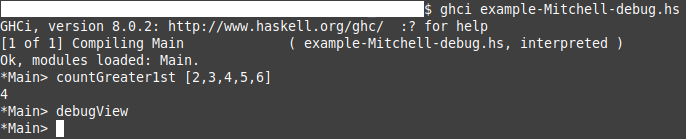
\includegraphics[scale=0.5]{pozivanje-mitchell.png}
\caption{Primer pozivanja ghci i debug putem terminala}
\end{center}
\end{figure}

Nakon što pozovemo bilo koju funkciju i ona se izvrši, ona zahvaljujući debug funkciji ostavlja trag- Komandom debugView pozivamo browser prozor koji nam prikazuje željene informacije. Druga opcija je da sa debugRun automatski izvršimo funkciju i pozovemo prozor.

\begin{figure}[h!]
\begin{center}
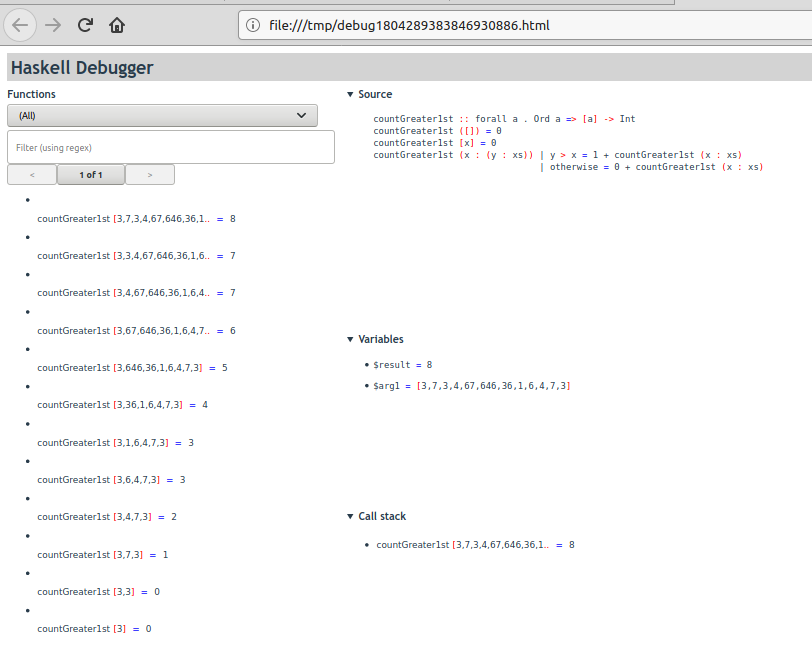
\includegraphics[scale=0.4]{mitchell-browser-pregled.png}
\caption{Prozor Debug-a nakon primene countGreater1st}
\end{center}
\end{figure}

Za svaku od levo navedenih funkcija koje predstavljaju call stack ovog programa možemo jasno videti argumente i rezultat, što nam omogućava pregledno debagovanje bilo kog Haskell programa.
Primetićemo da prvi primer radi kako treba, tj vraća 8 elementa veća od prvog. Probajmo sad ostale primere.

\begin{figure}[h!]
\begin{center}
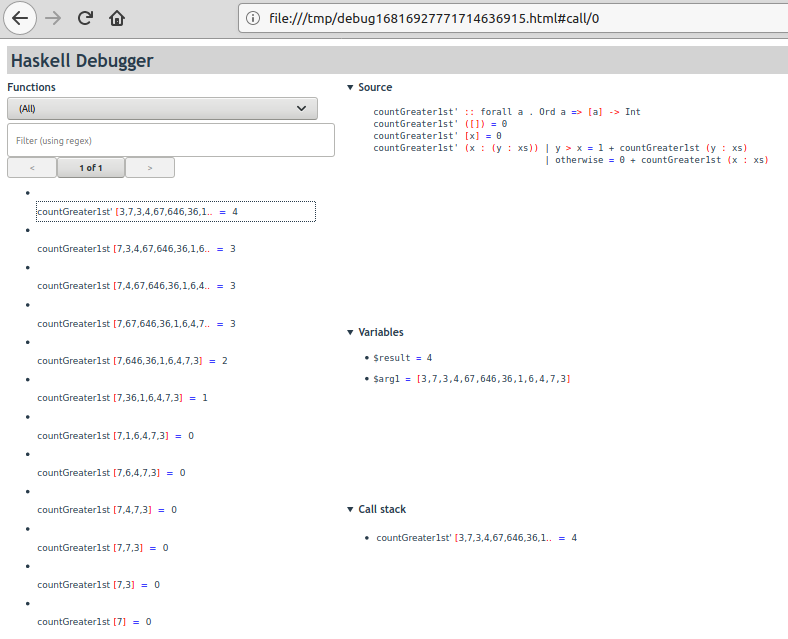
\includegraphics[scale=0.3]{mitchell-browser-pregled'.png}
\caption{Prozor Debug-a nakon primene countGreater1st'}
\end{center}
\end{figure}

Ovaj primer vraća rezultat 3. Na nama je da vidimo u čemu je problem. U levoj strani možemo videti sve funkcije koje su pozvane, što nam služi kao call stack programa. Prvi red predstavlja prvu pozvanu funkciju. Drugi red nam je sledeći poziv. Primetimo da je neobičan. Naš plan s ovom funkcijom je da nađemo broj elemenata veći od prvog, a izgleda da smo ga odbacili pri drugom pozivu.
Gore imamo programski kod funkcije i možemo pogledati šta je urađeno.
Kad je drugi element veći od prvog, mi rekurzivno pozivamo funkciju sa listom bez prvog elementa, i tako kroz ostale. Našli smo bug!

\begin{figure}[h!]
\begin{center}
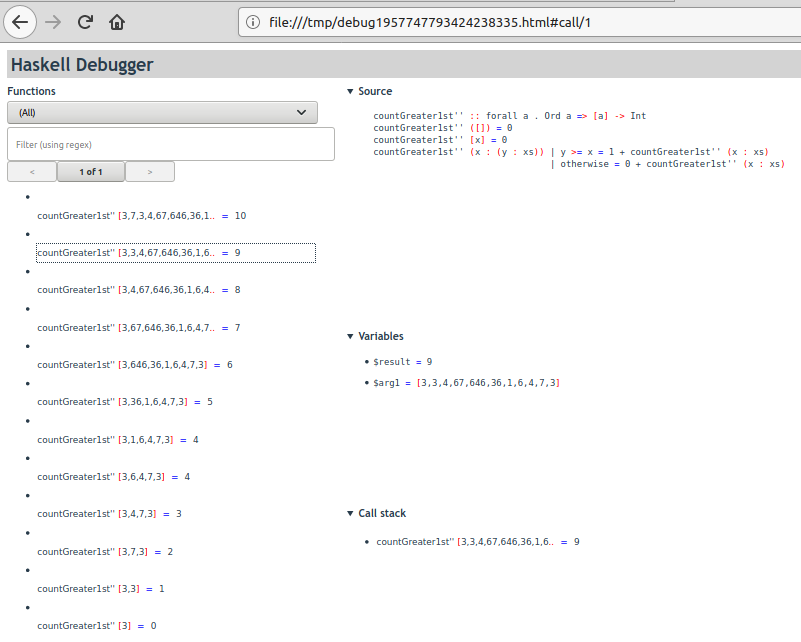
\includegraphics[scale=0.3]{mitchell-browser-pregled''.png}
\caption{Prozor Debug-a nakon primene countGreater1st'', izabrali smo drugi poziv da pogledamo}
\end{center}
\end{figure}

Dobijamo krajnji rezultat 10. Primetimo u drugom pozivu, gledajući call stack, da on vraća +1 za niz koji počinje sa 3,3. Gledajući kod funkcije primetimo da vraća +1 kada su jednaki brojevi. Bug je pronađen!

Ovo je u suštini kako se radi sa Debug-om. Jednostavan prozor gde se vidi manje-više sve što treba.

\subsection{Problemi debug-a}

Debug nije bez svojih problema. 
On koristi Show instance da bi prikazao vrednosti, što pravi probleme ako se program oslanja na lenjo izračunavanje, na primer kad imamo beskonačni niz. U tom slučaju program če najčešće da crash-uje ili se zaglavi u beskonačnoj petlji.

\subsection{Debug.Hoed}

Biblioteka građena na Debug i koja koristi TemplateHaskell, koja podržava lenjo izračunavanje i nudi jasan prikaz Call Stack-a. Primer kako izgleda prozor s njim se može videti \href{https://rawgit.com/pepeiborra/debug-hoed/master/example/quicksort.html}{ovde}. 
Za razliku od Debug, Debug.Hoed nema gorenavedenih problema. Važno je napomenuti da je Debug u eksperimentalnoj fazi, tako da će korisnici njega potencijalno imati drugih problema pri korišćenju.

Nažalost, nismo u mogućnosti da prikažemo praktičan primer sa Debug.Hoed usled problema sa zastarelom verzijom ghci koja se dobija preko apt repozitorijuma(8.0 umesto 8.2+)

\section{Engleski termini i citiranje}	
\label{sec:termini_i_citiranje}

Na svakom mestu u tekstu naglasiti odakle tačno potiču informacije. Uz sve novouvedene termine u zagradi naglasiti od koje engleske reči termin potiče. 

Naredni primeri ilustruju način uvođenja enlegskih termina kao i citiranje.

\begin{primer}
Problem zaustavljanja (eng.~{\em halting problem}) je neodlučiv \cite{haltingproblem}.
\end{primer}

\begin{primer}
Za prevođenje programa napisanih u programskom jeziku C može se koristiti GCC kompajler \cite{gcc}.
\end{primer}

\begin{primer}
 Da bi se ispitivala ispravost softvera, najpre je potrebno precizno definisati njegovo ponašanje \cite{laski2009software}. 
\end{primer}

Reference koje se koriste u ovom tekstu zadate su u datoteci {\em seminarski.bib}. Prevođenje u pdf format u Linux okruženju može se uraditi na sledeći način:
\begin{verbatim}
pdflatex TemaImePrezime.tex 
bibtex TemaImePrezime.aux 
pdflatex TemaImePrezime.tex 
pdflatex TemaImePrezime.tex 
\end{verbatim}
Prvo latexovanje je neophodno da bi se generisao {\em .aux} fajl. {\em bibtex} proizvodi odgovarajući {\em .bbl} fajl koji se koristi za generisanje literature. 
Potrebna su dva prolaza (dva puta pdflatex) da bi se reference ubacile u tekst (tj da ne bi ostali znakovi pitanja umesto referenci). Dodavanjem novih referenci potrebno je ponoviti ceo postupak.  











Broj naslova i podnaslova je proizvoljan. Neophodni su samo Uvod i Zaključak. Na poglavlja unutar teksta referisati se po potrebi. 
\begin{primer}
U odeljku \ref{sec:naslov1} precizirani su osnovni pojmovi, dok su zaključci dati u odeljku \ref{sec:zakljucak}.
\end{primer}

Još jednom da napomenem da nema razloga da pišete:
\begin{verbatim}
\v{s} i \v{c} i \'c ...
\end{verbatim}
Možete koristiti srpska slova
\begin{verbatim}
š i č i ć ... 
\end{verbatim}



\section{Slike i tabele}
\label{slike_i_tabele}

Slike i tabele treba da budu u svom okruženju, sa odgovarajućim naslovima, obeležene labelom da koje omogućava referenciranje. 

\begin{primer} Ovako se ubacuje slika. Obratiti pažnju da je dodato i 
\begin{verbatim}
\usepackage{graphicx}
\end{verbatim}

\begin{figure}[h!]
\begin{center}
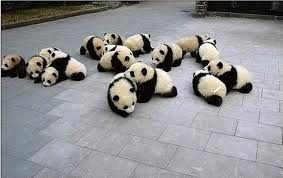
\includegraphics[scale=0.75]{panda.jpg}
\end{center}
\caption{Pande}
\label{fig:pande}
\end{figure}

Na svaku sliku neophodno je referisati se negde u tekstu. Na primer, na slici \ref{fig:pande} prikazane su pande. 
\end{primer}

\begin{primer} I tabele treba da budu u svom okruženju, i na njih je neophodno referisati se u tekstu. Na primer, u tabeli \ref{tab:tabela1} su prikazana različita poravnanja u tabelama.

\begin{table}[h!]
\begin{center}
\caption{Razlčita poravnanja u okviru iste tabele ne treba koristiti jer su nepregledna.}
\begin{tabular}{|c|l|r|} \hline
centralno poravnanje& levo poravnanje& desno poravnanje\\ \hline
a &b&c\\ \hline
d &e&f\\ \hline
\end{tabular}
\label{tab:tabela1}
\end{center}
\end{table}

\end{primer}

\section{K\^{o}d i paket listings}
Za ubacivanje koda koristite paket \textbf{listings}:
\url{https://en.wikibooks.org/wiki/LaTeX/Source_Code_Listings}

\begin{primer}
Primer ubacivanja koda za programski jezik Python dat je kroz listing \ref{simple}. Za neki drugi programski jezik, treba podesiti odgvarajući programski jezik u okviru defnisanja stila.
\end{primer}
\begin{lstlisting}[caption={Primer ubacivanja koda u tekst},frame=single, label=simple]
# This program adds up integers in the command line
import sys
try:
    total = sum(int(arg) for arg in sys.argv[1:])
    print 'sum =', total
except ValueError:
    print 'Please supply integer arguments'
\end{lstlisting}


\section{Prvi naslov}
\label{sec:naslov1}


Ovde pišem tekst. 
Ovde pišem tekst. 
Ovde pišem tekst. 
Ovde pišem tekst. 
Ovde pišem tekst. 
Ovde pišem tekst. 
Ovde pišem tekst. 
Ovde pišem tekst. 


\subsection{Prvi podnaslov}
\label{subsec:podnaslov1}

Ovde pišem tekst. 
Ovde pišem tekst. 
Ovde pišem tekst. 
Ovde pišem tekst. 
Ovde pišem tekst. 
Ovde pišem tekst. 
Ovde pišem tekst. 

\subsection{Drugi podnaslov}
\label{subsec:podnaslov2}

Ovde pišem tekst. 
Ovde pišem tekst. 
Ovde pišem tekst. 
Ovde pišem tekst. 
Ovde pišem tekst. 
Ovde pišem tekst. 


\subsection{... podnaslov}
\label{subsec:podnaslovN}

Ovde pišem tekst. 
Ovde pišem tekst. 
Ovde pišem tekst. 
Ovde pišem tekst. 
Ovde pišem tekst. 
Ovde pišem tekst. 

\section{n-ti naslov}
\label{sec:naslovN}

Ovde pišem tekst. 
Ovde pišem tekst. 
Ovde pišem tekst. 
Ovde pišem tekst. 
Ovde pišem tekst. 

\subsection{... podnaslov}
\label{subsec:podnaslovK}

Ovde pišem tekst. 
Ovde pišem tekst. 
Ovde pišem tekst. 
Ovde pišem tekst. 
Ovde pišem tekst. 

\subsection{... podnaslov}
\label{subsec:podnaslovM}

Ovde pišem tekst. 
Ovde pišem tekst. 
Ovde pišem tekst. 
Ovde pišem tekst. 
Ovde pišem tekst. 


\section{Zaključak}
\label{sec:zakljucak}

Ovde pišem zaključak. 
Ovde pišem zaključak. 
Ovde pišem zaključak. 
Ovde pišem zaključak. 
Ovde pišem zaključak. 
Ovde pišem zaključak. 
Ovde pišem zaključak. 
Ovde pišem zaključak. 
Ovde pišem zaključak. 
Ovde pišem zaključak. 
Ovde pišem zaključak. 
Ovde pišem zaključak. 


\addcontentsline{toc}{section}{Literatura}
\appendix
\bibliography{seminarski} 
\bibliographystyle{plain}

\appendix
\section{Dodatak}
Ovde pišem dodatne stvari, ukoliko za time ima potrebe.
Ovde pišem dodatne stvari, ukoliko za time ima potrebe.
Ovde pišem dodatne stvari, ukoliko za time ima potrebe.
Ovde pišem dodatne stvari, ukoliko za time ima potrebe.
Ovde pišem dodatne stvari, ukoliko za time ima potrebe.


\end{document}
